\documentclass[12pt]{article}

\usepackage{sbc-template}
\usepackage{graphicx,url}
\usepackage[utf8]{inputenc}
\usepackage[brazil]{babel}
\usepackage[latin1]{inputenc}  
\usepackage{xcolor}
\usepackage{caption}


\sloppy

\title{Desenvolvimento de um Aplicativo Web Progressivo\\Demonstrando os Princípios e Práticas de Criação de PWAs}

\author{João Vitor Lima Lago Santos, Luis Paulo da Silva Carvalho}

\address{Instituto Federal da Bahia (IFBA)\\
  Av. Sérgio Vieira de Melo, 3150 - Zabelê\\  
  Vitória da Conquista, Bahia, Brasil\\ 
  \email{joaovitorllsgm@gmail.com, luiscarvalho@ifba.edu.br}
}

\begin{document} 

\maketitle

\begin{abstract}
\textbf{Context}: the popularization of smartphones has allowed people all over the world to have access to different types of information and to interact with each other without geographic restrictions. Such devices are carried by the majority of the world's population, therefore, new technologies emerge and are improved, so that their users can better interact with them. Among the various existing technologies, progressive web applications or PWAs stand out, as they allow the creation or adaptation of web pages into mobile applications equipped with the capabilities of native apps and modern browsers, providing a better user experience and reducing costs with code maintenance. \textbf{Goal}: This article discusses the principles and best practices that govern this technology and aims to demonstrate them in the development of a progressive web application. \textbf{Method}: Therefore, we transformed a web application into a PWA through the evolution of its source code. \textbf{Results}: we equipped the final version of application with features relevant to PWAs, such as, responsive adaptation to different screen formats, application-like behavior, independent connectivity. \textbf{Conclusions}: We demonstrate that PWA is a skillful way to bring native mobile app behaviors to web applications with relatively low effort.

\end{abstract}
     
\begin{resumo} 
\textbf{Contexto}: a popularização de smartphones permitiu que pessoas por todo o planeta tenham acesso a diferentes formas de informação e que possam interagir entre si sem restrições geográficas. Considerando tal uso tão difundido, novas tecnologias emergem e são melhoradas. Entre as várias tecnologias existentes, destacamos as aplicações web progressivas, ou PWAs. Elas permitem a criação ou adaptação de páginas web como aplicativos móveis equipados com recursos de softwares nativos e também de navegadores web modernos. \textbf{Objetivo}: este trabalho discute os princípios e melhores práticas que governam esta tecnologia e foca em mostrá-los no desenvolvimento de aplicações web progressivas. \textbf{Método}: para tanto, neste trabalho, uma aplicação web foi transformada em uma PWA a partir da evolução de seu código fonte. \textbf{Resultado}: a versão final correspondeu à mesma aplicação web, mas dotada com recursos pertinentes ao universo de PWAs, tais como, por exemplo, adaptação responsiva a diferentes formatos de tela, comportamento semelhante a aplicativos, conectividade independente. \textbf{Conclusão}: demonstramos que PWA é uma via hábil para trazer para aplicações web comportamentos nativos de aplicativos móveis com esforço relativamente baixo.  
\end{resumo}

\section{Introdução}

Os dispositivos móveis estão cada vez mais presentes no cotidiano das pessoas, seja por conta da praticidade e portabilidade fornecidas, seja pela vasta quantidade de funcionalidades presentes, como aplicativos instalados pelas lojas de aplicativos, como por exemplo, o navegador Chrome, Uber e Netflix. Tal praticidade e portabilidade possibilitaram um grande aumento no uso da internet por meio dos smartphones, que segundo Roumeliotis e Tsekilas (2022), representou 79\% acessando a Internet por meio do dispositivo.

Devido ao crescente aumento nos acessos às páginas web, tecnologias correlatas ao desenvolvimento de aplicações web estão passando por constantes atualizações para melhor se encaixrem no dia a dia dos usuários. Visando superar algumas limitações encontradas em aplicativos para dispositivos móveis, tais como, consumo em excesso de recursos, limitações de plataformas ou sistemas operacionais específicos, foi desenvolvida uma nova visão chamada de PWA (\textit{Progressive Web Apps}, ou, em português, Aplicações Web Progressivas), que visa unir as capacidades de uma página web com as funcionalidades encontradas em dispositivos móveis. Este avanço conta com alguns princípios, por exemplo, o instalável, o linkável e o responsívo (os demais princípios se encontram na sessão 2.1).

Este trabalho seguiu um conjunto de passos, especificados na Figura 1, que vão desde a investigação da tecnologia de Aplicações Web Progressivas e sua aplicabilidade, entendendo seus princípios, conceitos e boas práticas através de um levantamento teórico, até a aplicação desses princípios no desenvolvimento de uma PWA baseada em uma prova de conceito, onde estes princípios foram exemplificados.

\begin{figure}[ht]
\centering
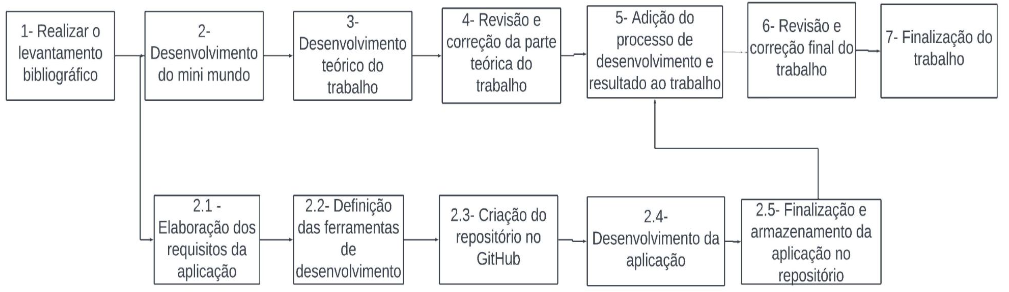
\includegraphics[width=1\textwidth]{imagens/processos.png}
\caption{Processos metodológicos}
\label{fig:processos}
\end{figure}

\section{Aplicações Web Progressivas} \label{sec:pwa}

Segundo Russel e Berrimam (2015), trata-se de um termo nomeado em 2015 pelo desenvolvedor do Chrome, Alex Russel, e pelo designer, Frances Berriman, em um artigo idealizando a tecnologia e seus princípios intitulado como “Aplicativos Web progressivos: escapando das guias sem perder a alma”. Tais aplicações não são empacotadas e implantadas em lojas, são apenas sites que receberam todas as "vitaminas certas", e que "os sites que desejam enviar notificações ou estar na tela inicial precisam conquistar esse direito". Tais afirmações elucidam algumas características e peculiaridades de PWAs. Neste caso, diferentemente dos aplicativos, uma PWA não se encontraria em lojas de aplicativos e deverá ser instalada por meio do site acessado. A partir do artigo original, foi determinado que Aplicações Web Progressivas são páginas web que possuem a capacidade de se comportarem como aplicativos em dispositivos móveis, compartilhando de recursos presentes nos dois ambientes. 

Segundo Doan (2019) Aplicações Web Progressivas são aplicações web que oferecem uma experiência nativa superior ao usuário usando os recursos mais recentes dos navegadores modernos. Tem-se, como exemplo, o modo de funcionamento offline, que, segundo Deviana et al. (2021), possibilita que uma PWA funcione offline ou com conexões de baixa qualidade, o que permite que uma PWA trabalhe independente do estado de conexão do dispositivo utilizado.

Um ponto interessante sobre as PWAs é que pode-se utilizar uma aplicação web já existente como base, conforme afirma Doan (2019), tanto novas aplicações quanto já existentes podem se tornar PWAs. A parte mais importante na criação de uma PWA reside no cumprimento de todos os seus princípios e práticas, pontos que serão abordados e que foram implementados na forma de uma prova de conceito ao longo deste trabalho.

\subsection{Princípios de uma PWA} \label{sec:principios}

Os princípios de PWA são a forma como as aplicações devem se comportar para que sejam consideradas uma PWA. Segundo [Berriman e Russel 2015], [ e Tsekilas 2022] e [Doan 2019] , uma PWA deve responder aos seguintes princípios:

\begin{enumerate}
    \item \textbf{Responsivo}: sendo adaptável a diferentes formatos de telas de dispositivos, permite que o site seja visualizado por dispositivos com diferentes resoluções de tela;
    \item \textbf{Conectividade independente}: permite que a aplicação funcione de forma offline com o uso dos \textit{service workers}. Utiliza scripts para um carregamento de arquivos gravados durante conexões anteriores (cache) durante momentos de falta de conectividade;
    \item \textbf{Semelhante a aplicativos}: adota o modelo de aplicativo para fornecer melhor navegação e interação. Permite que a página progressiva entregue uma melhor experiência de interface, escondendo funções disponíveis no navegador, como barra de endereço, abas de navegação e outras opções. Também faz uso de responsividade para melhor posicionar os elementos;
    \item \textbf{Novo}: deve realizar atualizações transparentes graças ao processo de atualização do \textit{service worker}. Por se tratar de uma única base de código e pelo fato do \textit{service worker} sempre buscar informações novas em momentos onde há conectividade, a PWA sempre estará disponível em sua versão mais atual;
    \item \textbf{Descobrivel}: são identificados como “aplicativos” por meio do \textit{web manifest} e o registro do \textit{service worker}, permitindo que os mecanismos de busca os encontrem. É por meio do \textit{web manifest} e do \textit{service worker} que uma aplicação web pode ser reconhecida como uma aplicação web progressiva e que possa ser instalada;
    \item \textbf{Re-engajável}: pode acessar funcionalidades do dispositivo para gerar re-engajamento do usuário. Por exemplo, através de notificações. Para tanto, deve ter acesso a recursos normalmente vistos em dispositivos móveis, tais como, vibração ou notificações, permitindo alertar o usuário sobre alterações ou novos conteúdos;
    \item \textbf{Instalável}: permite a adição de um ícone de acesso ao aplicativo na tela inicial do dispositivo.  Assim, o usuário acessa de forma mais fácil e dinâmica a página, sem ter que utilizar um navegador web;
    \item \textbf{Linkável}: são de fácil compartilhamento por meio de uma URL, através da qual é possível acessar o site desejado e posteriormente adicioná-lo à tela inicial do dispositivo.
\end{enumerate}

\subsection{Tecnologias usadas por uma PWA} \label{sec:tecnologias}

Aplicações PWA são desenvolvidas utilizando HTML, CSS, JavaScript e um arquivo JSON chamado de \textit{web manifest}. Tem foco principalmente no JavaScript, utilizando \textit{service workers} para permitir o comportamento de aplicativo e garantir a realização dos princípios descritos na Seção 2.1. Atualmente, existem  frameworks web que possuem a capacidade de desenvolver PWAs, tais como, por exemplo, o Vue.js, que será utilizado no desenvolvimento da prova de conceito alvo deste trabalho juntamente com a linguagem de programação, TypeScript\footnote{Link para acesso: https://www.typescriptlang.org/}. As próximas seções descrevem as tecnologias citadas com mais detalhes.

\subsubsection{Web Manifest} \label{sec:web_manifest}

O \textit{web manifest} é um arquivo do tipo .json ou .webmanifest que contém um conjunto de informações relevantes sobre a aplicação, conforme mostrado na Figura \ref{fig:web_manifest}\footnote{Versão completa no link: https://abrir.link/gRVBH}.

\begin{figure}[ht]
\centering
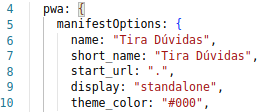
\includegraphics[width=.5\textwidth]{imagens/manifest.jpg}
\caption{Web Manifest}
\label{fig:web_manifest}
\end{figure}

É por meio destas informações que o navegador entende que uma aplicação é web progressiva e permite a sua instalação em um dispositivo móvel ou desktop. Cada atributo desse arquivo possui uma funcionalidade, que pode ser definida da seguinte forma:

\begin{enumerate}
    \item \textbf{name}: define o nome da aplicação e será utilizada no momento da instalação, definindo o nome abaixo do ícone, que estará presente na tela inicial do dispositivo;
    \item \textbf{short\_name}: define um nome curto ou apelido do aplicativo. É utilizado quando a propriedade name possui muitos caracteres, enquanto define um nome mais compacto para o  aplicativo;
    \item \textbf{start\_url}: define a URL que é carregada quando o aplicativo é inicializado em um dispositivo. Por exemplo, o arquivo index.html, contendo a home page da aplicação;
    \item \textbf{display}: define a forma de exibição da aplicação, permitindo ao desenvolvedor promover uma experiência do usuário mais consistente;
    \item \textbf{theme\_color}: define o tema da cor da aplicação.
\end{enumerate}

\subsubsection{Service Worker} \label{sec:service_worker}

Um \textit{service worker} é um \textit{script} javascript, que executa em segundo plano e é responsável por gerenciar funcionalidades presentes em uma PWA: o envio de notificações por meio de \textit{Push Notifications}, mensagens que aparecem na tela do celular, avisando o usuário sobre alguma novidade, seja uma nova mensagem do WhatsApp ou um aplicativo que recebeu novo conteúdo, geolocalização, vibração e a sincronização da página. 
  
É composto principalmente por funções que são responsivas a eventos específicos, como o \textit{installing}, que permite definir uma lógica de programação para quando a PWA for instalada ou o \textit{fetch}, chamada sempre que ocorre o recarregamento da página, sendo responsável por buscar os arquivos requisitados pela aplicação através de requisições ou carregá-los  a partir da memória cache, caso os dados tenham sido previamente armazenados. Resumidamente, o \textit{service worker} é um \textit{script} essencial para o funcionamento de uma PWA, pois possui toda a lógica relacionada ao seu comportamento em um dispositivo móvel.

\subsubsection{Vue.js} \label{sec:vuejs}

Segundo Chau (2022) o Vue\footnote{Link para acesso: https://vuejs.org/} é um \textit{framework} javascript para a construção de interfaces de usuário. Utilizando HTML, CSS, JavaScript ou TypeScript e um modelo de programação orientado a componentes, a tecnologia auxilia no desenvolvimento de interfaces. Como um \textit{framework}, o objetivo do Vue é garantir um desenvolvimento padronizado, ágil e consistente de novas aplicações.

O Vue conta com um conjunto de bibliotecas e ferramentas que auxiliam no seu desenvolvimento como o vue-router\footnote{Link para acesso: https://router.vuejs.org/}, para o gerenciamento e controle de rotas, o pinia\footnote{Link para acesso:  https://pinia.vuejs.org/}, para o controle de estado de dados em memória, o bootstrap\footnote{Link para acesso: https://getbootstrap.com/}, o tailwind\footnote{Link para acesso: https://tailwindcss.com/} e o quasar\footnote{Link para acesso: https://quasar.dev/}, bibliotecas de componentes que possibilitam um melhor desenvolvimento de interfaces de forma padronizada. 

\section{Prova de conceito} \label{sec:tira_duvidas}

Com o objetivo de aplicar os princípios da PWA, foi desenvolvido uma aplicação chamada TiraDúvidas. O projeto baseia-se em um sistema web criado durante um evento conhecido como NLW (\textit{Next Level Week}) realizado pela Rocketseat\footnote{Link para acesso: https://www.rocketseat.com.br/}, uma \textit{coding school}, cuja missão é capacitar pessoas que buscam se profissionalizar na programação.

O TiraDúvidas tem, como objetivo, a criação de uma plataforma de salas para o compartilhamento de perguntas, onde é possível acessar uma sala existente ou criar uma nova. Após acessar ou criar uma sala é possível ler as perguntas enviadas pelos membros e escolher marca-las como lidas ou excluí-las.

É importante ressaltar que, originalmente, o projeto foi criado com o intuito de ser somente uma aplicação web, não possuindo recursos PWA (responsividade, por exemplo). Portanto, é um bom exemplo para demonstrar a aplicação dos princípios de PWA na prática. Logo abaixo serão apresentados todos os princípios que foram aplicados ao Tira Dúvidas.

\subsection{Responsividade} \label{sec:responsividade}

A responsividade é a capacidade de um site ou aplicativo de adaptar seus elementos ao tamanho da interface. Segundo Chau (2022), “design web responsivo refere-se ao uso do HTML e Folhas de Estilo em Cascata (CSS) para criar uma interface de usuário ideal independente de como a página é  acessada”. É um recurso que impacta na exibição de um site na busca realizada por ferramentas de busca, conforme exemplificado na Figura \ref{fig:responsividade}, que exibe, à esquerda, uma versão desktop e, à direita, uma versão mobile.

\begin{figure}[ht!]
\centering
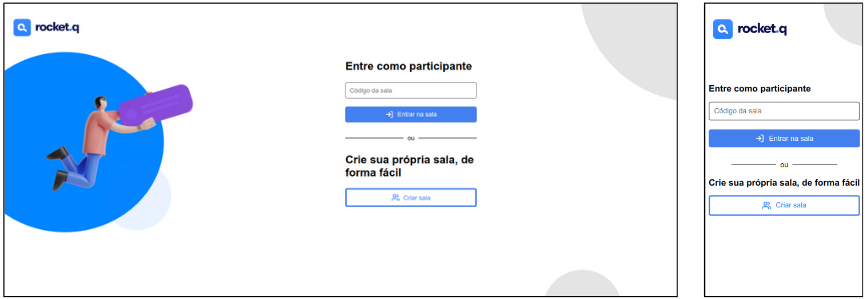
\includegraphics[width=.9\textwidth]{imagens/responsividade.jpg}
\caption{Tela Inicial em Diferentes Resoluções de Tela}
\label{fig:responsividade}
\end{figure}

Para que a responsividade na Figura 5 seja aplicada, faz-se o uso de \textit{media queries}\footnote{Link para acesso: https://abrir.link/Lakim}. Com esse recurso é possível definir estilos específicos para resoluções de tela diferentes com poucas linhas de código, conforme exemplificado na Figura \ref{fig:media}\footnote{Versão completa no link: https://abrir.link/yGqOM}.

\begin{figure}[ht!]
\centering
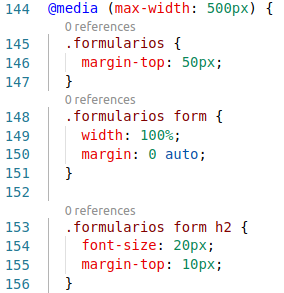
\includegraphics[width=0.4\textwidth]{imagens/media.jpg}
\caption{Uso do Media Queries}
\label{fig:media}
\end{figure}


\subsection{Cache} \label{sec:cache}

O cache é uma funcionalidade dos navegadores que permite o armazenamento de recursos de um site, tais como, arquivos HTML, CSS, JavaScript e imagens. Segundo Tamire (2019) o desenvolvedor pode pré-cachear ou cachear certos arquivos e assets a fim de permitir que a aplicação web seja exibida em uma situação quando o aplicativo está offline. Em conjunto com o \textit{service worker}, o cache é responsável pela exibição da aplicação PWA em momentos de falta de conectividade. 

\begin{figure}[ht!]
\centering
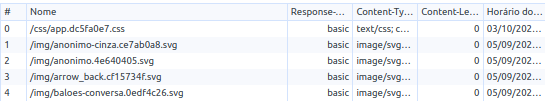
\includegraphics[width=0.8\textwidth]{imagens/cache.jpg}
\caption{Uso de Armazenamento em Cache}
\label{fig:cache}
\end{figure}

A Figura \ref{fig:cache} apresenta arquivos que foram compilados e gravados para uso posterior pelo Vue e o workbox, um conjunto de módulos que simplificam o roteamento e o armazenamento em cache comuns do \textit{service worker} para controle do cache. Por meio deles, uma versão de pré-cache do TiraDúvidas é criada. Esse cache inicial guarda informações importantes para o funcionamento da aplicação, como os estilos, \textit{scripts} e imagens usadas no momento da execução \textit{offline}.

\subsection{Instalável} \label{sec:instalavel}

Este recurso permite que o TiraDúvidas simule alguns dos comportamentos de um aplicativo. Segundo Tamire (2019), uma PWA funciona como um aplicativo nativo uma vez que o usuário navega na aplicação ou instala o link na tela inicial. Existem dois arquivos fundamentais para a instalação e funcionamento de uma PWA, o \textit{Web Manifest} (Figura \ref{fig:web_manifest}) e o \textit{service worker} apresentado na Figura \ref{fig:service_worker}.

\begin{figure}[ht!]
\centering
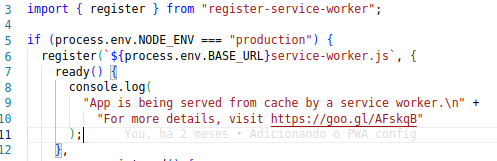
\includegraphics[width=0.7\textwidth]{imagens/service_worker.jpg}
\caption{Arquivo de Registro do Service Worker}
\label{fig:service_worker}
\end{figure}

O \textit{service worker}, mostrado na Figura \ref{fig:service_worker}\footnote{Versão completa no link: https://abrir.link/39g15}, é o \textit{script} responsável por disponibilizar algumas funcionalidades: (i) a manipulação da memória cache, (ii) acesso a APIs nativas do dispositivo, (iii) atualização de informações em segundo plano e (iv) funcionamento \textit{offline}. 

Como resultado da implementação dos princípios, o TiraDúvidas se torna instalável em um dispositivo, conforme demonstra o ícone presente na Figura \ref{fig:instalavel}, e seu conteúdo se torna acessável.

\begin{figure}[ht!]
\centering

\includegraphics[width=0.3\textwidth]{imagens/instalavel.png}
\caption{Ícone da PWA no Dispositivo}
\label{fig:instalavel}
\end{figure}

\subsection{Linkável} \label{sec:linkavel}

Este recurso permite que as PWAs sejam compartilhadas por meio de ULRs ao invés de uma loja de aplicativos, exibindo uma opção de compartilhar ou de abrir no navegador.

A partir do link o usuário terá acesso ao site do aplicativo e poderá utilizar de suas funcionalidades sem a necessidade de instalação, somente instalando se assim desejar.

% \begin{table}[ht]
% \centering
% \caption{Variables to be considered on the evaluation of interaction
%   techniques}
% \label{tab:exTable1}
% 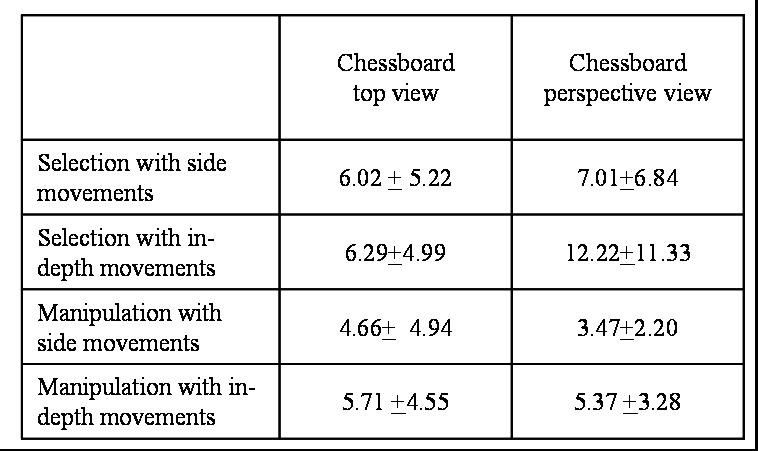
\includegraphics[width=.7\textwidth]{table.jpg}
% \end{table}

\subsection{Descobrível} \label{sec:descobrivel}

Permite que o site seja reconhecido como uma PWA pelos navegadores e ferramentas de busca. Como resultado uma opção de instalação aparecerá nas opções de navegadores, \textit{e.g}, Chromium ou Google Chrome.

Vale ressaltar que caso o \textit{Web Manifest} e o \textit{Service Worker} não forem corretamente adicionados a opção que aparecerá no lugar será a de adicionar a tela inicial, porém a mesma não possui os recursos de uma PWA como o acesso \textit{offline}.

\subsection{Semelhante a Aplicativo} \label{sec:semelhante_aplicativo}

Tem como objetivo trazer uma melhor experiência ao usuário, ocultando funcionalidades presentes no navegador, como barra de busca, abas de navegação e opções de configuração.

\subsection{Atualizações transparentes} \label{sec:atualizacoes}

Permite que a PWA seja atualizada em tempo real, sem a necessidade de realizar uma atualização por meio da loja de aplicativos. A PWA é capaz de detectar atualizações existentes e solicitar que o usuário recarregue o aplicativo ou simplesmente acessando o mesmo em momentos de conectividade, trazendo assim as novas funcionalidades adicionadas.

Ao final da implementação dos princípios, com o objetivo de melhor elucidar o uso e manter um registro sobre o uso da aplicação para estudos futuros, foi elaborado um vídeo explicativo, apresentando os conceitos aplicados no Tira Dúvidas. O link\footnote{https://youtu.be/CAbSQNp1E0c} pode ser acessado através do QRCode da Figura \ref{fig:video_funcionamento}.

\begin{figure}[ht!]
\centering

\includegraphics[width=0.2\textwidth]{imagens/video_funcionamento.jpg}
\caption{Vídeo explicativo sobre o software}
\label{fig:video_funcionamento}
\end{figure}

\section{Contribuições} \label{sec:contribuicoes}

Ao final da pesquisa e do desenvolvimento deste trabalho, foram obtidas versões parciais e uma final dos código-fontes. Na versão inicial\footnote{https://abrir.link/6it4I} uma foi adicionado o código fonte do Tira Dúvidas, possuindo as funcionalidades: entrar em uma sala, adicionar comentários, marcá-los como lidos, removê-los e copiar o código da sala. Neste primeiro momento, o site ainda não tinha a responsividade implementada.

\begin{figure}[ht!]
\centering

\includegraphics[width=0.2\textwidth]{imagens/codigo_nao_responsivo.jpg}
\caption{Versão inicial do Software (Sem Responsividade)}
\label{fig:codigo_nao_responsivo}
\end{figure}

Posteriormente, foi criada uma versão responsiva. Esta versão teve como objetivo aplicar os princípios da responsividade para que o software se adeque a resoluções de tela presentes nos smartphones.

\begin{figure}[ht!]
\centering

\includegraphics[width=0.2\textwidth]{imagens/codigo_responsivo.jpg}
\caption{Versão Responsiva do Software}
\label{fig:codigo_responsivo}
\end{figure}

Foi decidido manter duas versões do Tira Dúvidas, uma sem responsividade e outra com responsividade para que  os dois códigos-fonte servissem como material didático sobre a aplicação deste tipo de princípio (responsividade).

A versão final do projeto, cujo o link\footnote{https://abrir.link/ZmdeP} do código-fonte pode ser acessado através do QRCode que se encontra na Figura \ref{fig:versao_final}, contém a implementação, com sucesso, dos seguintes princípios: acesso offline, instalável, linkável, descobrível, semelhante a aplicativo e atualização transparente.

\begin{figure}[ht!]
\centering

\includegraphics[width=0.2\textwidth]{imagens/versao_final.jpg}
\caption{Versão Final}
\label{fig:versao_final}
\end{figure}

A versão online do projeto possibilita acessar e testar as funcionalidades e conceitos apresentados ao longo deste trabalho. O link\footnote{https://tira-duvidas-render.onrender.com/} para acesso se encontra na Figura \ref{fig:pwa_online}.

\begin{figure}[ht!]
\centering

\includegraphics[width=0.2\textwidth]{imagens/pwa_online.jpg}
\caption{Versão Online}
\label{fig:pwa_online}
\end{figure}

Ao final do trabalho foi realizada uma palestra para os alunos da disciplina, Interface Homem-Máquina (IHM), do curso de Bacharelado em Sistemas de Informação do IFBA, Campus Vitória da Conquista. A mesma foi importante para a disciplina, porque os conceitos abordados e praticados pelo autor principal desta pesquisa (responsividade e usabilidade em desenvolvimento web) também são vistos ao longo do semestre letivo da referida disciplina.

\section{Trabalhos Relacionados} \label{sec:correlatos}

Os próximos parágrafos contém uma investigação do estado da arte das PWAs e seus princípios.

Doan (2019) aborda a teoria por trás das Aplciações Web Progressivas, abrindo uma discussão acerca dos benefícios da tecnologia sobre outras existentes, como por exemplo, as aplicações nativas e híbridas, além de apresentar um exemplo de aplicação de uma PWA básica, demonstrando princípios de uma PWA, como o instalável e o acesso offline.

Em uma avaliação acerca das necessidades de um fluxo de reservas para companhias aéreas, Marques (2022) traz uma investigação sobre as capacidades da PWA, buscando entender seus pontos fortes e fracos em relação a uma aplicação nativa. Também disponibilizou recursos para que empresas avaliem se uma PWA é adequada às suas necessidades sobre a satisfação dos seus clientes, realizando o desenvolvimento de um protótipo, aplicando os princípios de responsividade e acesso offline.

Em Tamire (2019), é realizado um estudo acerca da possibilidade do uso de PWAs e o desenvolvimento de uma aplicação chamada de Relógio Anual. A  aplicação conta com recursos como uso offline, instalável e carregamento rápido. O estudo também conta com uma avaliação, como o acesso offline e performance.

Em Rensena (2020), é realizada, por meio de revisão bibliográfica e análise experimental, um estudo de diversos aspectos de uma PWA, como por exemplo: compatibilidade, desempenho, segurança, privacidade e o impacto em usuários e negócios. Para os testes de compatibilidade, uma validação por diferentes navegadores foi realizada avaliando diferentes aspectos, tais como, o funcionamento de \textit{service worker}, \textit{web manifest}, capacidade de adição a tela inicial e uso \textit{offline}. 

Em um estudo acerca da acessibilidade de PWAs para pessoas com deficiência, Roumeliotis e Tsekilas (2022) avaliam o quão acessível uma PWA é e quais as suas limitações. Para a elaboração deste estudo, 20 PWAs e 20 sites não PWAs foram analisados. Como resultado, foi avaliado que, apesar das limitações atuais, as PWAs oferecem aos usuários uma liderança em performace, otimização dos mecanismos de pesquisa e acessibilidade. Portanto, possuem espaço para futuras pesquisas centradas no ser humano e na acessibidade.

O Tira Dúvidas, aplicação web usada como prova de conceito neste trabalho e que é apresentado na Seção 3, aborda diversos princípios de uma PWA citados anteriormente e outros, conforme mostra a Tabela \ref{fig:comparativo}. Desta forma, este trabalho investiga, pelo menos, mais dois princípios que não foram observados pelos trabalhos aqui apontados.

\begin{table}[h]        
    \centering
    \begin{tabular}{|c|c|c|}\hline
      Princípios   &  Tira Dúvidas & Outras aplicações \\ \hline
      Responsividade  & X & X \\ \hline
      Acesso \textit{offline} & X & X \\ \hline
      Instalável & X & X \\ \hline
      Linkável & X & X \\ \hline
      Descobrível & X & X \\ \hline
      Semelhante a aplicativo & X & \\ \hline
      Atualização transparente & X & \\ \hline
      Re-engajável & & \\ \hline
\end{tabular}
\caption{Comparação de princípios aplicados}
\label{fig:comparativo}
\end{table}

\section{Conclusões e Trabalhos Futuros} \label{sec:conclusoes}

As PWAs são uma forma prática, ágil e econômica de desenvolvimento de aplicações web, \textit{mobile} e \textit{desktop}, pois permite que os usuários usufruam da mesma experiência em ambos os ambientes, além de poupar esforços no desenvolvimento do \textit{software}, utilizando do mesmo código fonte para duas frentes distintas, evitando duplicação de trabalho e manutenção. 

O Tira Dúvidas, um site para criação de salas para envio e compartilhamento de perguntas, visa exemplificar como os princípios e práticas, abordados e elucidados durante a revisão teórica, podem ser utilizados para que uma aplicação web nova ou já existente se adapte a essa tecnologia sem muitas dificuldades e conflitos, superando barreiras tecnológicas e encontrando espaço no nicho dos aplicativos nativos. É importante ressaltar que o Tira Dúvidas é somente um exemplo de aplicação destes conceitos, sendo possível todo e qualquer site ser aprimorado para uma PWA.
  
Sobre trabalhos futuros, uma possibilidade seria a avaliação de usabilidade de outros recursos não 
citados neste artigo, como, por exemplo, a geolocalização, acesso a câmera, sistema de arquivos do dispositivo e envio de notificações, sobre este último ponto, foi tentado a inclusão do mesmo no Tira Dúvidas, porém, por conta dos limites de prazo não foi possível aplicá-lo. Outra opção seria a implementação de uma PWA em um site que realize requisições a APIs de terceiros, permitindo avaliar a viabilidade do uso da tecnologia e seu desempenho em sites como redes sociais, plataformas de \textit{streaming} ou blogs de notícias, onde existe um grande tráfego de informações.

\bibliographystyle{sbc}
\bibliography{bibliografia}

\nocite{*}

\end{document}
